% Options for packages loaded elsewhere
\PassOptionsToPackage{unicode}{hyperref}
\PassOptionsToPackage{hyphens}{url}
\PassOptionsToPackage{dvipsnames,svgnames,x11names}{xcolor}
%
\documentclass[
  letterpaper,
  DIV=11,
  numbers=noendperiod]{scrartcl}

\usepackage{amsmath,amssymb}
\usepackage{iftex}
\ifPDFTeX
  \usepackage[T1]{fontenc}
  \usepackage[utf8]{inputenc}
  \usepackage{textcomp} % provide euro and other symbols
\else % if luatex or xetex
  \usepackage{unicode-math}
  \defaultfontfeatures{Scale=MatchLowercase}
  \defaultfontfeatures[\rmfamily]{Ligatures=TeX,Scale=1}
\fi
\usepackage{lmodern}
\ifPDFTeX\else  
    % xetex/luatex font selection
  \setmainfont[]{Inter}
  \setsansfont[]{Inter}
\fi
% Use upquote if available, for straight quotes in verbatim environments
\IfFileExists{upquote.sty}{\usepackage{upquote}}{}
\IfFileExists{microtype.sty}{% use microtype if available
  \usepackage[]{microtype}
  \UseMicrotypeSet[protrusion]{basicmath} % disable protrusion for tt fonts
}{}
\makeatletter
\@ifundefined{KOMAClassName}{% if non-KOMA class
  \IfFileExists{parskip.sty}{%
    \usepackage{parskip}
  }{% else
    \setlength{\parindent}{0pt}
    \setlength{\parskip}{6pt plus 2pt minus 1pt}}
}{% if KOMA class
  \KOMAoptions{parskip=half}}
\makeatother
\usepackage{xcolor}
\usepackage{soul}
\setlength{\emergencystretch}{3em} % prevent overfull lines
\setcounter{secnumdepth}{5}
% Make \paragraph and \subparagraph free-standing
\ifx\paragraph\undefined\else
  \let\oldparagraph\paragraph
  \renewcommand{\paragraph}[1]{\oldparagraph{#1}\mbox{}}
\fi
\ifx\subparagraph\undefined\else
  \let\oldsubparagraph\subparagraph
  \renewcommand{\subparagraph}[1]{\oldsubparagraph{#1}\mbox{}}
\fi

\usepackage{color}
\usepackage{fancyvrb}
\usepackage{tikz}
\newcommand{\VerbBar}{|}
\newcommand{\VERB}{\Verb[commandchars=\\\{\}]}
\DefineVerbatimEnvironment{Highlighting}{Verbatim}{commandchars=\\\{\}}
% Add ',fontsize=\small' for more characters per line
\usepackage{framed}
\definecolor{shadecolor}{RGB}{241,243,245}
\newenvironment{Shaded}{\begin{snugshade}}{\end{snugshade}}
\newcommand{\AlertTok}[1]{\textcolor[rgb]{0.68,0.00,0.00}{#1}}
\newcommand{\AnnotationTok}[1]{\textcolor[rgb]{0.37,0.37,0.37}{#1}}
\newcommand{\AttributeTok}[1]{\textcolor[rgb]{0.40,0.45,0.13}{#1}}
\newcommand{\BaseNTok}[1]{\textcolor[rgb]{0.68,0.00,0.00}{#1}}
\newcommand{\BuiltInTok}[1]{\textcolor[rgb]{0.00,0.23,0.31}{#1}}
\newcommand{\CharTok}[1]{\textcolor[rgb]{0.13,0.47,0.30}{#1}}
\newcommand{\CommentTok}[1]{\textcolor[rgb]{0.37,0.37,0.37}{#1}}
\newcommand{\CommentVarTok}[1]{\textcolor[rgb]{0.37,0.37,0.37}{\textit{#1}}}
\newcommand{\ConstantTok}[1]{\textcolor[rgb]{0.56,0.35,0.01}{#1}}
\newcommand{\ControlFlowTok}[1]{\textcolor[rgb]{0.00,0.23,0.31}{#1}}
\newcommand{\DataTypeTok}[1]{\textcolor[rgb]{0.68,0.00,0.00}{#1}}
\newcommand{\DecValTok}[1]{\textcolor[rgb]{0.68,0.00,0.00}{#1}}
\newcommand{\DocumentationTok}[1]{\textcolor[rgb]{0.37,0.37,0.37}{\textit{#1}}}
\newcommand{\ErrorTok}[1]{\textcolor[rgb]{0.68,0.00,0.00}{#1}}
\newcommand{\ExtensionTok}[1]{\textcolor[rgb]{0.00,0.23,0.31}{#1}}
\newcommand{\FloatTok}[1]{\textcolor[rgb]{0.68,0.00,0.00}{#1}}
\newcommand{\FunctionTok}[1]{\textcolor[rgb]{0.28,0.35,0.67}{#1}}
\newcommand{\ImportTok}[1]{\textcolor[rgb]{0.00,0.46,0.62}{#1}}
\newcommand{\InformationTok}[1]{\textcolor[rgb]{0.37,0.37,0.37}{#1}}
\newcommand{\KeywordTok}[1]{\textcolor[rgb]{0.00,0.23,0.31}{#1}}
\newcommand{\NormalTok}[1]{\textcolor[rgb]{0.00,0.23,0.31}{#1}}
\newcommand{\OperatorTok}[1]{\textcolor[rgb]{0.37,0.37,0.37}{#1}}
\newcommand{\OtherTok}[1]{\textcolor[rgb]{0.00,0.23,0.31}{#1}}
\newcommand{\PreprocessorTok}[1]{\textcolor[rgb]{0.68,0.00,0.00}{#1}}
\newcommand{\RegionMarkerTok}[1]{\textcolor[rgb]{0.00,0.23,0.31}{#1}}
\newcommand{\SpecialCharTok}[1]{\textcolor[rgb]{0.37,0.37,0.37}{#1}}
\newcommand{\SpecialStringTok}[1]{\textcolor[rgb]{0.13,0.47,0.30}{#1}}
\newcommand{\StringTok}[1]{\textcolor[rgb]{0.13,0.47,0.30}{#1}}
\newcommand{\VariableTok}[1]{\textcolor[rgb]{0.07,0.07,0.07}{#1}}
\newcommand{\VerbatimStringTok}[1]{\textcolor[rgb]{0.13,0.47,0.30}{#1}}
\newcommand{\WarningTok}[1]{\textcolor[rgb]{0.37,0.37,0.37}{\textit{#1}}}

\providecommand{\tightlist}{%
  \setlength{\itemsep}{0pt}\setlength{\parskip}{0pt}}\usepackage{longtable,booktabs,array}
\usepackage{calc} % for calculating minipage widths
% Correct order of tables after \paragraph or \subparagraph
\usepackage{etoolbox}
\makeatletter
\patchcmd\longtable{\par}{\if@noskipsec\mbox{}\fi\par}{}{}
\makeatother
% Allow footnotes in longtable head/foot
\IfFileExists{footnotehyper.sty}{\usepackage{footnotehyper}}{\usepackage{footnote}}
\makesavenoteenv{longtable}
\usepackage{graphicx}
\makeatletter
\def\maxwidth{\ifdim\Gin@nat@width>\linewidth\linewidth\else\Gin@nat@width\fi}
\def\maxheight{\ifdim\Gin@nat@height>\textheight\textheight\else\Gin@nat@height\fi}
\makeatother
% Scale images if necessary, so that they will not overflow the page
% margins by default, and it is still possible to overwrite the defaults
% using explicit options in \includegraphics[width, height, ...]{}
\setkeys{Gin}{width=\maxwidth,height=\maxheight,keepaspectratio}
% Set default figure placement to htbp
\makeatletter
\def\fps@figure{htbp}
\makeatother

\newfontfamily\sectionfont[Color=000000]{Inter} \newfontfamily\subsectionfont[Color=000000]{Inter} \newfontfamily\subsubsectionfont[Color=000000]{Inter} \addtokomafont{section}{\sectionfont} \addtokomafont{subsection}{\subsectionfont} \addtokomafont{subsubsection}{\subsubsectionfont} \usepackage{fvextra} \usepackage{svg} \DefineVerbatimEnvironment{Highlighting}{Verbatim}{breaklines,commandchars=\\\{\}}
\KOMAoption{captions}{tableheading}
\makeatletter
\makeatother
\makeatletter
\makeatother
\makeatletter
\@ifpackageloaded{caption}{}{\usepackage{caption}}
\AtBeginDocument{%
\ifdefined\contentsname
  \renewcommand*\contentsname{Table of contents}
\else
  \newcommand\contentsname{Table of contents}
\fi
\ifdefined\listfigurename
  \renewcommand*\listfigurename{List of Figures}
\else
  \newcommand\listfigurename{List of Figures}
\fi
\ifdefined\listtablename
  \renewcommand*\listtablename{List of Tables}
\else
  \newcommand\listtablename{List of Tables}
\fi
\ifdefined\figurename
  \renewcommand*\figurename{Figure}
\else
  \newcommand\figurename{Figure}
\fi
\ifdefined\tablename
  \renewcommand*\tablename{Table}
\else
  \newcommand\tablename{Table}
\fi
}
\@ifpackageloaded{float}{}{\usepackage{float}}
\floatstyle{ruled}
\@ifundefined{c@chapter}{\newfloat{codelisting}{h}{lop}}{\newfloat{codelisting}{h}{lop}[chapter]}
\floatname{codelisting}{Listing}
\newcommand*\listoflistings{\listof{codelisting}{List of Listings}}
\makeatother
\makeatletter
\@ifpackageloaded{caption}{}{\usepackage{caption}}
\@ifpackageloaded{subcaption}{}{\usepackage{subcaption}}
\makeatother
\makeatletter
\@ifpackageloaded{tcolorbox}{}{\usepackage[skins,breakable]{tcolorbox}}
\makeatother
\makeatletter
\@ifundefined{shadecolor}{\definecolor{shadecolor}{rgb}{.97, .97, .97}}
\makeatother
\makeatletter
\makeatother
\makeatletter
\makeatother
\ifLuaTeX
  \usepackage{selnolig}  % disable illegal ligatures
\fi
\IfFileExists{bookmark.sty}{\usepackage{bookmark}}{\usepackage{hyperref}}
\IfFileExists{xurl.sty}{\usepackage{xurl}}{} % add URL line breaks if available
\urlstyle{same} % disable monospaced font for URLs
\hypersetup{
  pdftitle={GSMST CyberDragons Yearlong Proposal},
  pdfauthor={Anish Goyal; Andrew Zeng; Bibek Bhattarai},
  colorlinks=true,
  linkcolor={blue},
  filecolor={Maroon},
  citecolor={Blue},
  urlcolor={Blue},
  pdfcreator={LaTeX via pandoc}}

\title{GSMST CyberDragons Yearlong Proposal}
\author{Anish Goyal \and Andrew Zeng \and Bibek Bhattarai}
\date{}

\begin{document}
\maketitle
\begin{tikzpicture}[overlay,remember picture]
  \node[anchor=center, opacity=0.3] at ([yshift=-2cm]current page.center) {
\includegraphics[width=2\paperwidth]{CyberDragons.png}};
\end{tikzpicture}
\ifdefined\Shaded\renewenvironment{Shaded}{\begin{tcolorbox}[boxrule=0pt, sharp corners, enhanced, breakable, borderline west={3pt}{0pt}{shadecolor}, frame hidden, interior hidden]}{\end{tcolorbox}}\fi

\renewcommand*\contentsname{Table of Contents}
{
\hypersetup{linkcolor=}
\setcounter{tocdepth}{6}
\tableofcontents
\begin{tikzpicture}[overlay,remember picture]
  \node[anchor=center, opacity=0.3] at ([yshift=-2cm]current page.center) {
\includegraphics[width=2\paperwidth]{CyberDragons.png}};
\end{tikzpicture}
}
\newpage{}

\hypertarget{list-of-competitions}{%
\section{List of Competitions}\label{list-of-competitions}}

Here is a list of competitions that GSMST CyberDragons will participate
in for the entire school year with their competition dates. This will
also cover some insights we will gain from participating in these
competitions in the field of cybersecurity and when we should start
preparing for said competition.

\hypertarget{cyberpatriot}{%
\subsection{CyberPatriot}\label{cyberpatriot}}

CyberPatriot is AFA's signature defensive cybersecurity competition
where you have to blah blah blah blah. Yeah ok we got it. It's basically
all of our meetings in the first 2 months of the year, then we kinda
move on to broader topics. And we gotta register our teams before July 1
to get a 20\% discount, but we don't actually have to pay anything until
November 1. But also according to Parv you have to pay to make the
teams, so maybe we tell Ms.~Rachkovskiy to do some magic: log into the
mainframe and do some hacking to make five teams without paying until
November but still receive the discount. During peak competition season
we might need to reserve a FLEX period if people want it so yea.

\hypertarget{cyberstart-america}{%
\subsection{CyberStart America}\label{cyberstart-america}}

So basically some guys in the United Kingdom made this cybersecurity
platform with a bunch of random problems on it right. and now they
expanded their reach to the United States, but since Americans
\emph{Hate} cybersecurity and won't Participate without some of that
good old dinero, they are offering cash prize for winners! This
competition is asynchronous and lasts from October to April, so
basically the entire year. we are bsaically just gonna encourage
everyone \emph{HEY GO CYBERSTART GO CYBERSTART} for the entire year and
then \st{we} they get free monies.

\hypertarget{cyber-skylines-national-cyber-league-ncl}{%
\subsection{Cyber Skyline's National Cyber League
(NCL)}\label{cyber-skylines-national-cyber-league-ncl}}

Cyber Skyline's National Cyber League (NCL) is a virtual cybersecurity
competition and training platform. It is designed to provide
participants, including students and professionals, with hands-on
experience and practical skills in various cybersecurity disciplines.
The NCL features a series of challenges that simulate real-world
scenarios, allowing participants to develop and demonstrate their
expertise in areas such as network security, cryptography, web
application security, log analysis, and more. The NCL follows a gamified
approach, where participants compete individually or in teams to solve a
series of challenges within a given timeframe. These challenges are
designed to assess participants' technical knowledge, critical thinking,
problem-solving abilities, and ability to work under pressure. The
platform offers different difficulty levels, ranging from introductory
to advanced, catering to participants with varying skill levels (Can you
tell I ChatGPT'ed this yet?).

There are two competitions offered in the NCL event: the individual game
and the team game. The individual game takes place from March 31 to
April 2, and you can register whenever you want for the individual game,
even during the competition period itself. For the team game, the
competition period is April 14 to April 16, and you have to register
starting In January By April 13 by 23:59 PM (Wait, why did I say PM if
it's in military time?). It costs \$35 per team for a max of two teams.
We could recruit two teams and make each team member pay a hefty little
fine along with that. And there's 7 members max per team. This
competition also focuses on log analysis, network traffic analysis, etc.

\hypertarget{lockheed-martins-cyberquest}{%
\subsection{Lockheed Martin's
CyberQuest}\label{lockheed-martins-cyberquest}}

\href{https://www.lockheedmartin.com/en-us/who-we-are/communities/cyber-quest.html}{\emph{CyberQuest}} is a cloud-based competition created by Lockheed Martin cybersecurity engineers. It will take place on \textbf{March 4}, and registration closes on \textbf{Februrary 3}. There will be multi-step intrustion, stenography, reverse engineering, full OS hack, packet capture, and web exploitation. They will provide users with desktops that have Kali \& Windows installed, both in-person and online.

\begin{itemize}
\tightlist
\item
  It's free
\item
  Two methods: virtual and in-person

  \begin{itemize}
  \tightlist
  \item
    Going in-person requires a field trip to \st{Ohio} Orlando, Florida,
    since that's the nearest location for the competition.
  \end{itemize}
\item
  There is a 2 team limit for virtual and in-person each (4 max).
\end{itemize}

\hypertarget{us-cyber-challenge-cyber-quests}{%
\subsection{US Cyber Challenge: Cyber
Quests}\label{us-cyber-challenge-cyber-quests}}

\emph{Cyber Quests} is a online competition allowing participants to
demonstrate their knowledge in a variety of information security realms.
The main benefit of this competition is that it has a niche quiz (the
entire competition is basically a quiz) that deals \emph{a lot} with
networking. Registration opens in the end of January, and the
competition is from mid-February to the end of March. Registration
closes at the end of the competition. It's also free of cost. There are
no ``teams'' for this either; you have to create an account and
participate individually and asynchronously, similar to \emph{CyberStart
America.}

\hypertarget{technology-student-associations-cybersecurity-event}{%
\subsection{Technology Student Association's Cybersecurity
Event}\label{technology-student-associations-cybersecurity-event}}

Ok I might be crazy to promote TSA since they are like our rivals, but
hear me out. Their cybersecurity event is an asynchronous jeopardy-style
CTF challenge that is essentially a ripoff of picoCTF. The idea here is
the following: if we can somehow siphon CyberDragons members into this
event, we can smurf on everyone else in the country and basically get
first place in the national TSA conference and SLC. The event
registration begins at the beginning of the school year and ends
whenever TSA events end.

\hypertarget{dicectf}{%
\subsection{DiceCTF}\label{dicectf}}

\href{https://ctf.dicega.ng/}{\emph{DiceCTF}} is an annual
jeopardy-style CTF competition hosted in \textbf{early February}
\href{https://github.com/dicegang/dicectf-2023-challenges}{every year}.
The prize pool is \$5000, and it is open to all students.

\hypertarget{asis-ctf}{%
\subsection{ASIS CTF}\label{asis-ctf}}

\href{https://asisctf.com/}{\emph{ASIS CTF}} is an annual jeopardy-style
CTF competition organized by the ASIS (Academy for Skills and
Information Security) team. There is no restriction on the number of
team members, and the problems include: general security infomration
(trivia), web hacking, modern cryptography, exploit, forensics, reverse
engineering, steganography, \emph{etc.} The qualification round is in
\textbf{late September} and finals are in \textbf{December}.

\hypertarget{uxe5ngstromctf}{%
\subsection{ÅngstromCTF}\label{uxe5ngstromctf}}

\href{https://angstromctf.com/}{\emph{ÅngstromCTF}} is another
jeopardy-style CTF competition hosted by team Ångstrom. It holds a focus
on binary exploitation, cryptography, reverse engineering, and web
exploitation, with a few miscellanous questions. It occurs in
\textbf{late April}.

\hypertarget{csaw-ctf}{%
\subsection{CSAW CTF}\label{csaw-ctf}}

\href{https://www.csaw.io/ctf}{\emph{CSAW CTF}} is one of the oldest and
biggest CTFs. Jeopardy-style CTF, this competition is for students who
are trying to break into the field of security, as well as for advanced
students and industry professionals who want to practice their skills.
The qualifiers take place from \textbf{September 8 to September 10}, but
high schoolers cannot go past the qualifier round.

\hypertarget{tjctf}{%
\subsection{TJCTF}\label{tjctf}}

\href{https://tjctf.org/}{\emph{TJCTF}} is a jeopardy-style CTF
competition that takes place in \textbf{late May} (probably after school
is out/during finals). The categories in this competition are:
cryptography, binary exploitation, reverse engineering, web
exploitation, forensics, \emph{etc.}

\hypertarget{la-ctf}{%
\subsection{LA CTF}\label{la-ctf}}

\href{https://lactf.uclaacm.com}{\emph{LA CTF}} is a jeopardy-style CTF
competition hosted by UCLA. There is no size limit on teams, and
non-UCLA students must compete in the Open division. The competition
consists of a variety of competitive cybersecurity challenges in
addition to relaxed events like typing competitions. It takes place in
\textbf{mid-February} for 42 hours. What we think is really cool about
this CTF competition specifically is that there are also prizes awarded
for the best write ups to the challenges of the competition, and write
ups include video walkthroughs. So, if we really wanted to tryhard this
CTF, we could just make a bunch of YouTube videos with really high
production value and potentially get some prizes from doing that alone.
But the prizes for winning the \emph{actual} competition are \$500,
\$300, \$200, and \$100 for 1st, 2nd, 3rd, and 4/5th place,
respectively. Another really cool thing about this competition is that
there are going to be speakers on the UCLA campus streamed live for all
the virtual participants. A notable name is \emph{John Hammond}, who has
his own YouTube channel for picoCTF stuff.

\newpage{}

\hypertarget{cyberdragons-syllabus}{%
\section{CyberDragons Syllabus}\label{cyberdragons-syllabus}}

It is time for my favorite part, the cyberdragons syllabus, which I
would have made whether it was required or not. We have already talked
about what we want to cover on the syllabus for the entire year, but
none of us have the leisure to start drafting a syllabus at this time
(we cba), so we will probably work on it towards the end of July.
Therefore, the deadline for the syllabus will be \textbf{August 1}.

\hypertarget{syllabus-research} of the
meeting participants came prepared with three topics to cover for the
syllabus and why those topics were important for future competitions and
the broader aspect of cybersecurity. All we have to do now is figure out
when we want to cover these topics and how we could structure our lesson
plans for them, which we'll do in another meeting towards the end of
July.

\hypertarget{anish-goyals-research}{%
\subsubsection{Anish Goyal's Research}\label{anish-goyals-research}}

\begin{itemize}
\tightlist
\item
  \textbf{Web Application Security}

  \begin{itemize}
  \tightlist
  \item
    Discuss common vulnerabilities in web applications, such as
    cross-site scripting (XSS), SQL injection, and cross-site request
    forgery (CSRF). Explain techniques like input validation and secure
    coding practices to mitigate these risks, or how to exploit them.
    This is important for picoCTF's \emph{Web Exploitation} module and
    Cyberpatriot's \emph{Boeing Web Challenge} that will have an
    approximately 99.9999\% chance of being a part of next year's
    competition.
  \end{itemize}
\item
  \textbf{AES (Advanced Encryption Standard)}

  \begin{itemize}
  \tightlist
  \item
    It's the most widely used symmetric encryption algorithm and is
    employed in various applications, including securing sensitive data,
    protecting communication channels, and ensuring confidentiality in
    data storage. Throughout the years, we have seen forensic questions
    about AES in CyberPatriot and even some \emph{Cryptography} and
    \emph{Reverse Engineering} challenges in last year's picoCTF
    competition that involved AES encryption/decryption and salting.
  \end{itemize}
\item
  \textbf{Network Time Protocol (NTP) Security}

  \begin{itemize}
  \tightlist
  \item
    We want to learn how to security configure the NTP kernel module to
    synchronize system clocks with trusted time sources and prevent
    time-based attacks, such as replay attacks or certificate validity
    issues. This is an important aspect of kernel hardening for Linux
    systems that is typically overlooked throughout the CyberPatriot
    competition, and we could even throw in some networking systemctl
    safety measures in there (e.g.~Martian packet tracing and preventing
    IPv4 wait-time assassination attacks).
  \end{itemize}
\end{itemize}

\hypertarget{bibek-bhattarais-research}{%
\subsubsection{Bibek Bhattarai's
Research}\label{bibek-bhattarais-research}}

\begin{itemize}
\tightlist
\item
  \textbf{Hacking Tools}

  \begin{itemize}
  \tightlist
  \item
    Teach how to use commonly found exploiting software like Jack the
    Ripper, Wireshark, BurpSuite, and pwntools.
  \end{itemize}
\end{itemize}

\begin{Shaded}
\begin{Highlighting}[numbers=left,,]
\BuiltInTok{Error}\NormalTok{ at }\BuiltInTok{Line} \DecValTok{59} \OperatorTok{(}\BuiltInTok{NullPointerException}\OperatorTok{:} \BuiltInTok{Class} \StringTok{"Bibek"}\NormalTok{ with }\BuiltInTok{Attributes} \StringTok{"Research Topic 2"}\NormalTok{ and }\StringTok{"Research Topic 3"}\NormalTok{ Not Found}\OperatorTok{)}
\end{Highlighting}
\end{Shaded}

\hypertarget{andrew-zengs-research}{%
\subsubsection{Andrew Zeng's Research}\label{andrew-zengs-research}}

\begin{itemize}
\tightlist
\item
  \textbf{General Encryption}

  \begin{itemize}
  \tightlist
  \item
    This topic is commonly covered through a unit within CSP, but to
    serve as a further step, CyberDragons can offer to focus on this
    topic towards the beginning of the year in order to serve as a
    transition from those who were initially piqued by the confines of
    the CSP curriculum and teach them about the various different
    encryption and decryption methods used by ethical hackers and
    cybersecurity defenders.
  \end{itemize}
\item
  \textbf{Network Defense}

  \begin{itemize}
  \tightlist
  \item
    Although one can work to troubleshoot a cybersecurity problem on
    their own, it's generally important for those to use and apply the
    tools already provided to them. This lesson could range from
    covering various firewalls, access control, how a network is split
    and can pertain specifically to Windows Server, Windows, as I
    remember from CyberPatriot.
  \end{itemize}
\item
  \textbf{Scripting (PowerShell and whatnot)}

  \begin{itemize}
  \tightlist
  \item
    Scripting is integral (I got calc PTSD reading that Cursed Word)
    pertaining to cybersecurity as it can often automate the process of
    breaking into or fixing common breaches that occur in the world.
  \end{itemize}
\end{itemize}

\newpage{}

\hypertarget{cyberpatriot-applications}{%
\section{CyberPatriot Applications}\label{cyberpatriot-applications}}

Just like last school year, we plan to have an application process for
CyberPatriot CyberDragons. However, we will be diversifying the process
a little bit this year.

\hypertarget{the-main-application}{%
\subsection{The Main Application}\label{the-main-application}}

Here is how the \emph{main} CyberPatriot application for this year will
work:\\

\begin{enumerate}
\def\labelenumi{\arabic{enumi})}
\tightlist
\item
  There will be three qualifying practice images that members must
  complete to the best of their ability in a two-week timeframe: one
  Windows, one Ubuntu, and one Fedora. The theme for each of these
  images will be PORTAL:
\end{enumerate}

\begin{figure}

{\centering 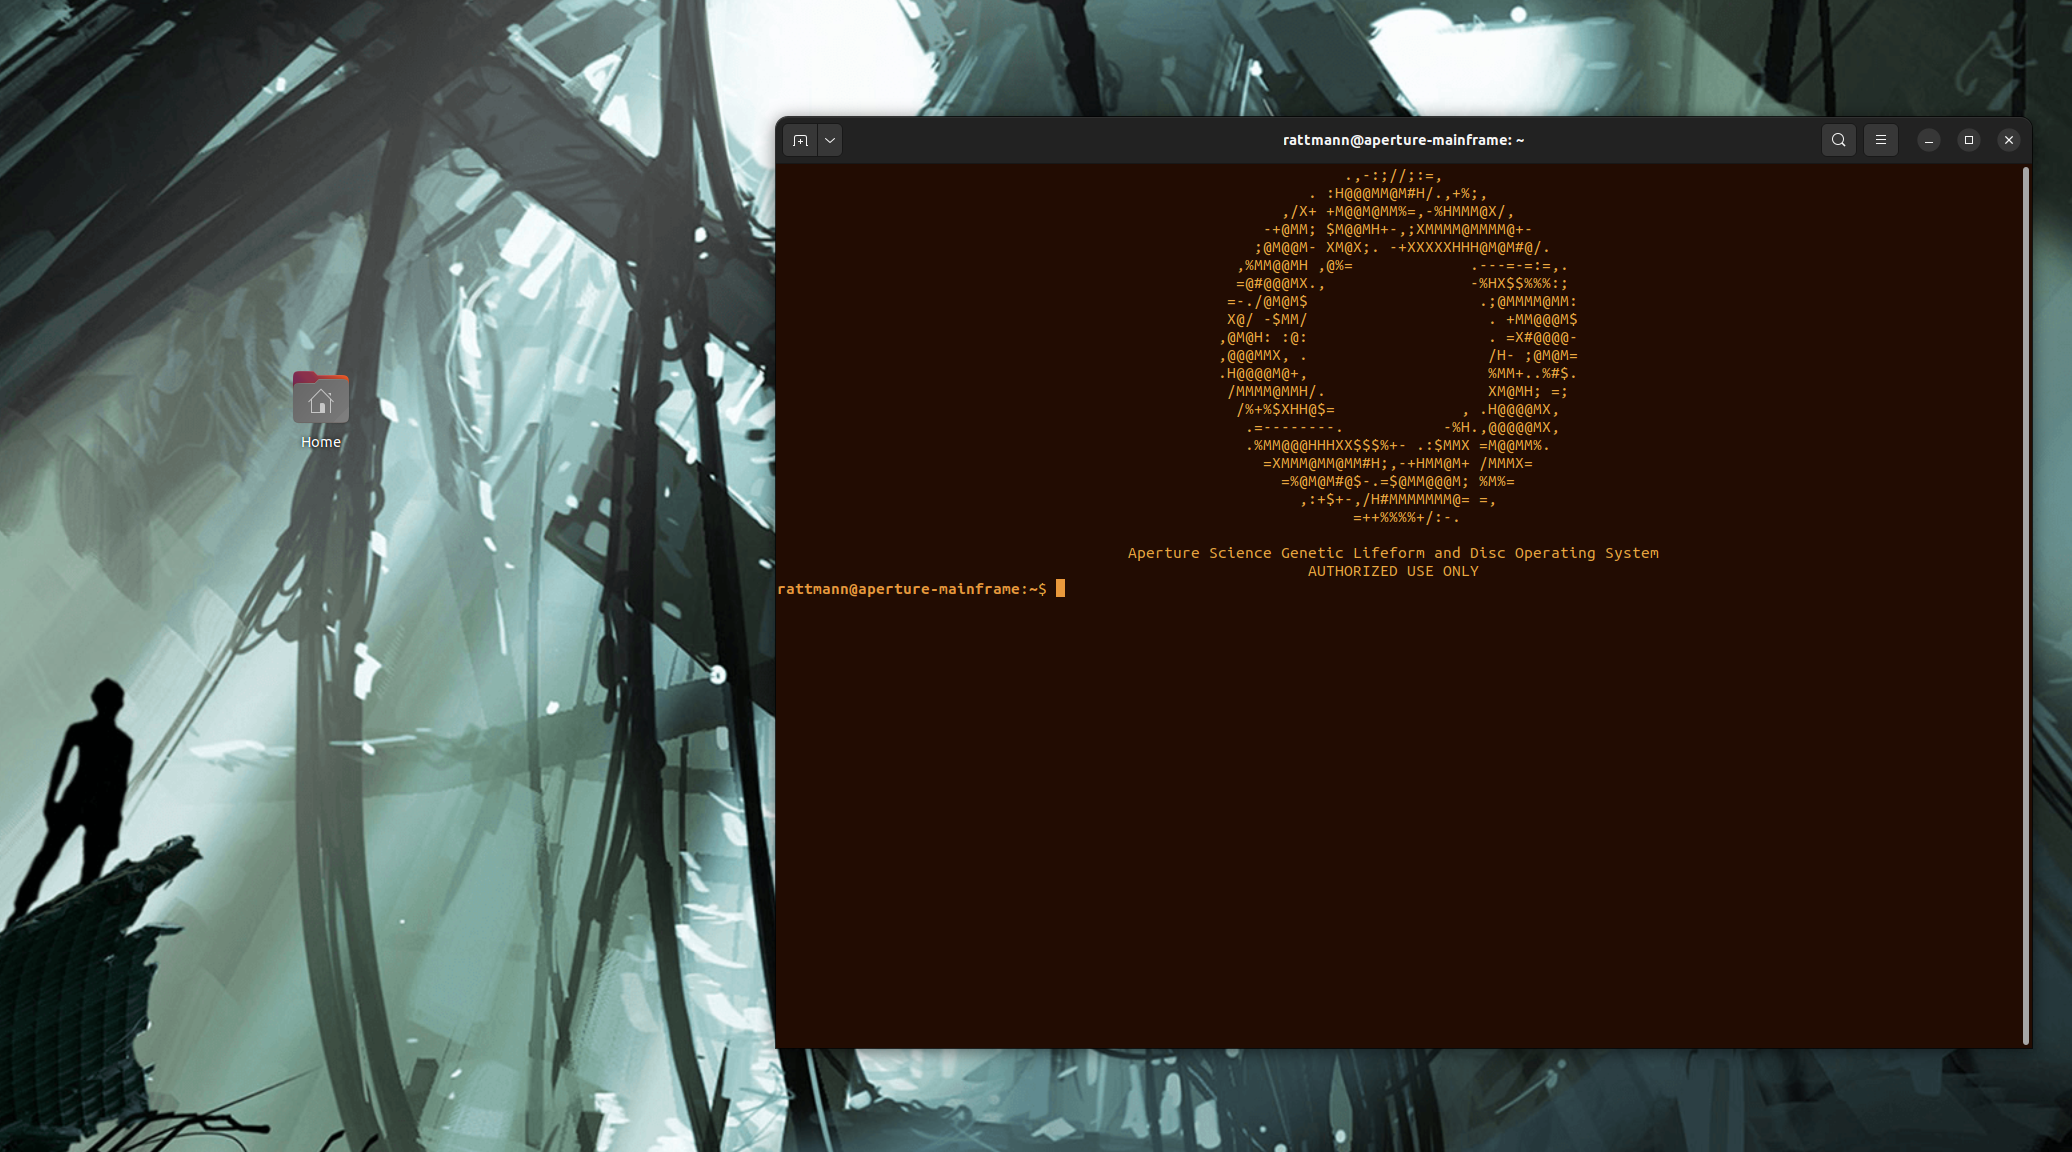
\includegraphics{PORTAL.png}

}

\caption{A portal-themed virtual image}

\end{figure}

\begin{enumerate}
\def\labelenumi{\arabic{enumi})}
\setcounter{enumi}{1}
\tightlist
\item
  Once the applicants are satisfied with their progress (or if the two
  week deadline is approached), they must email a screenshot of their
  results to the GSMST CS Club email address, which I cba to get right
  now.\\
\item
  The applicants have to fill out a Google Form with short-answer
  questions to complete that are completely qualitative in nature. I
  hate fluffy questions like ``Why do you want to be here!'' and ``What
  experience do you have to offer!'' so I will make sure the questions
  are a lot better than those piece of trash. And I'm not gonna kill the
  applicants either: completing three practice images is already a lot
  of work, so I'm only gonna ask for them to write like 2 sentences
  minimum per question.\\
\item
  Make sure the applicant can pay the \$30 fee. On the Google Form, make
  sure they check a box that says ``I can pay the \$30 fee or ask
  Ms.~Rachkovskiy for a fee waiver if I need one.'' Of course, this fee
  does not apply for members of Team Phi, and we're not even gonna say
  that the \$30 is ``a donation.''
\end{enumerate}

\hypertarget{team-phi-application}{%
\subsection{Team Phi Application}\label{team-phi-application}}

Next year, if an applicant wants to be in Team Phi, they have to fill
out another Google Form! You might be wondering why we are making
prospective members of Team Phi fill out another Google Form \emph{in
addition} to the main CyberPatriot application if our mission is to
promote equity---well, the idea of another application is not to deter
prospective Team Phi members; it is simply that we anticipate that the
demand to get into Team Phi is gonna be so high next year (because of
the nature that it is free of cost) that we have to make getting into
Team Phi a separate application process altogether. We wanted to
remove the requirement that all members of Team Phi has to be members of
Girls Who Code, but after a vote of our esteemed Girls Who Code club officers, it was decided against. Therefore, all new incoming Team Phi applicants \textit{must} be members of Girls Who Code.

\hypertarget{cyberpatriot-team-leader-application}{%
\subsection{CyberPatriot Team Leader
Application}\label{cyberpatriot-team-leader-application}}

Last year, we had a team leader for each team in CyberPatriot, and all
of them were club officers. This year, especially since we only have
three cybersecurity officers, we have opted to allow CyberPatriot
participants \emph{themselves} apply for leadership positions. This
gives each team a degree of autonomy to which they can function, and a
chance for CyberDragons members to put something nice on their resume
(e.g.~``I led a CyberPatriot team to semifinals!!! Omg, I'm the GOAT of
all time!''). But of course---like all great things in our lives---there
will be a Google Form allotted (alloted?) for this purpose. And five
people will be accepted, one for each team. Oh, and they have to be a
returning member because there is no way in \st{hell} heck that we are
going to make someone with no CyberPatriot experience a leader. You need
to know what you are doing, and it is a huge responsibility to drive
people in the competition, cause if your team is lost, your team is
doomed to fail.

\hypertarget{cyberpatriot-team-distribution}{%
\section{CyberPatriot Team
Distribution}\label{cyberpatriot-team-distribution}}

With the addition of Team Zeta next year, we have to consider how we are
going to distribute members across all five of our CyberPatriot teams.
Well, actually, the solution here is simple. Most, if not all of our
CyberPatriot members last year filled out the \emph{returning member
Google Form}. This means that we can reserve a spot for them on their
original teams without moving them whatsoever (assuming they actually go
through the aforementioned application process). Then, we put all the
newbies in any spots not reserved for members that filled out the
returning form.

\hypertarget{a-new-approach-to-teaching}{%
\section{A New Approach to Teaching}\label{a-new-approach-to-teaching}}

GSMST CS Club's cybersecurity department was a massive success last
year, but there was one massive pitfall: we taught students
cybersecurity concepts to excel in competitions, but they often didn't
retain the information taught at these seminars. However, they
\emph{did} remember cybersecurity approaches from messing around in
virtual machines and scoring points. This year, we aim to take a more
hands-on approach to cybersecurity. We will no longer have seminars---we
will have workshops. Not only will this will solve our main problem last
year---disappointment from students who did not get into CyberPatriot or
joined later in the year, since we will be in more than triple the
amount of competitions---it will also solve the problem of audience
retention, since we will be taking a learn \emph{by} doing approach
instead of a learn \emph{then} doing approach.

So what does this mean, and how do we plan to implement this? Firstly,
this means that our workshops will not be curated specifically for a
competition. It will be generic cybersecurity concepts that will be
useful in preparing for various competitions, but not something labeled
as a ``CyberPatriot'' or ``PicoCTF'' meeting. And in order to implement
interactivity, we can use virtual desktop software on a 24/7 server
(managed by my old laptop) that will control any virtual machine for
people to mess around with, CyberPatriot style! This gives us the
infrastructure for mini practice images for students to tackle during
workshops and even networking challenges with WireShark and Cisco Packet
Tracer. We can also use platforms with response validation like Desmos
to generate interactive lessons for students.

\newpage{}

\hypertarget{discord-server-revamp}{%
\section{Discord Server Revamp}\label{discord-server-revamp}}

Since we're no longer GSMST CyberPatriot CyberDragons, we're just gonna
call ourselves GSMST CyberDragons, since we're in multiple competitions.
And now we got ourselves an awesome logo:

\begin{figure}

{\centering 
\includegraphics[width=0.5\textwidth,height=\textheight]{CyberDragons.png}

}

\caption{GSMST CyberDragons logo made by the esteemed Yubo Cao}

\end{figure}

The CyberDragons server revamp was done on July 1, 2023. We reformatted the \#resources channel to be a compendium of resources, tidied up the CyberPatriot channels, and added a server logo. In the upcoming future, we plan on making an Instagram for CyberDragons.

\newpage{}

\hypertarget{cyberdragons-curated-competitions}{%
\section{CyberDragons-Curated
Competitions}\label{cyberdragons-curated-competitions}}

We, as a team, discussed the feasibility of having in-school competitions for CyberDragons. The only problem is that our schedule is so jampacked that we probably wouldn't figure out a date with everyone available, nor garner enough interest to do it. Therefore, \textbf{everything is tentatively canceled}, but we'll leave the following information here just in case: 
The CyberDragons administrative team will create competitions to inspire
camaraderie (I hope that's how you spell it, I cba to check) among
teammates and prepare for actual competitions.The competitions we
propose are the following:

\hypertarget{cyberpatriot-mock-competition}{%
\subsection{CyberPatriot Mock
Competition}\label{cyberpatriot-mock-competition}}

This is a competition that we plan to have sometime between the first
and second CyberPatriot round. We cannot have a mock competition between
the second round and the state round because of midterms and conflicts
with the SAT, but a mock competition between the first two rounds is
definitely doable. I don't have an exact month for this right now, but
it would have to take place on a Saturday for 6 hours between the first
two rounds, and we would have 3 images (Windows, Ubuntu, and Fedora) and
a Cisco Packet Tracer Lab (.pka file).

\hypertarget{in-house-infosecurity-competition}{%
\subsection{In-House Infosecurity
Competition}\label{in-house-infosecurity-competition}}

We are gonna host a competition that is a copy of CyberPatriot without
calling it \emph{``CyberPatriot''} (Genius, I know right?). It's gonna
take place on a Saturday for 6 hours in April, which surprisingly has a
ton of dates to schedule things. It will be \emph{Lord of the Rings}
themed with the same 3 images (but no Cisco Packet Tracer this time,
good riddance!).

\hypertarget{cisco-packet-tracer}{%
\section{Cisco Packet Tracer}\label{cisco-packet-tracer}}

Speaking of Cisco Packet Tracer (my favorite part of CyberPatriot), we
have taken measures to ensure that Cisco will not be overshadowed by the
rest of the competition next year. AFA is actually really nice and tells
us which NetAcad modules are covered on the quizzes for each
CyberPatriot round ahead of time, so we can prepare some slideshow
presentations/notes for people to read through in order to \st{cram} get
ready for that aspect of the competition. There's also a ton of mentors
that I'm on the look out for. I've scouted LinkedIn and found a couple
of mentors that might be interested in helping us, such as Binh Tran
(Who you might know as a Gwinnett Technical College professor). There's
also Mr.~Hong, who coaches ACSL, who apparently has Cisco and networking
experience, despite not using packet tracer himself.

\hypertarget{picoctf}{%
\section{picoCTF}\label{picoctf}}

Last year, the picoCTF meetings faced a lack of attendance: in fact, it
was our lowest attending seminar on average \textbf{by far}. It seemed
that the popularity and attention given to CyberPatriot overshadowed
picoCTF, making it difficult for people to make it to the Thursday
meetings. Unfortunately, this resulted in a disappointing turnout.
Recognizing this issue, we decided to remove picoCTF as a regular
meeting day altogether.

However, we devised a solution to ensure that picoCTF received the
attention it deserved during the competition season this year. Rather
than holding regular meetings on Thursdays, a few Fridays would be
dedicated specifically to picoCTF. This adjustment would provide an
opportunity for participants to focus on the competition and engage with
picoCTF-related activities. Additionally, a couple of FLEX periods could
be allocated for picoCTF, allowing students to further immerse
themselves in the preparation and training required for the competition.

In the past, we've always referred to our Friday meetings as
\emph{CyberPatriot} meetings:

\begin{figure}

{\centering 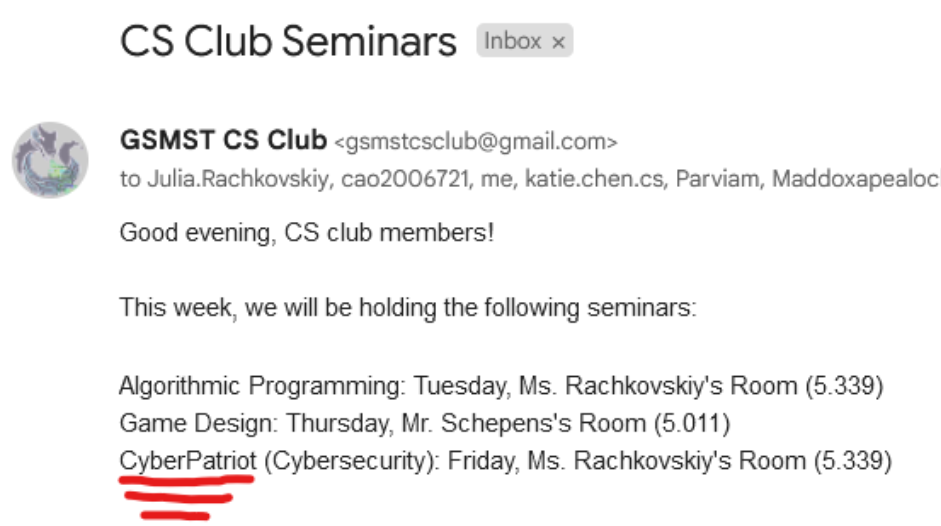
\includegraphics[width=0.8\textwidth,height=\textheight]{email.png}

}

\caption{An email from last year containing our seminar schedule. Notice
how it says ``CyberPatriot.''}

\end{figure}

However, a lot of the content that we covered in our ``CyberPatriot''
meetings weren't even related to the actual CyberPatriot
\emph{competition}---they were just cybersecurity concepts in general.
Furthermore, a lot of the topics covered in picoCTF overlapped with the
topics we brought up in CyberPatriot in general. Therefore, it's better
to just merge the two into a new seminar called \emph{``Cybersecurity''}
every Friday, covering concepts in both offensive and defensive
security.

\hypertarget{budgeting}{%
\section{Budgeting}\label{budgeting}}

GSMST CS Club is broke. And we incurred a lot of debt because of
CyberPatriot last year. But now, we have a sustainable plan to make sure
that doesn't happen again.

We have two competitions this year that require payment:

\begin{itemize}
\tightlist
\item
  \textbf{CyberPatriot:} \$160 * 4 teams = \$640
\item
  \textbf{NCL:} \$35 * 3 teams = \$105

  \begin{itemize}
  \tightlist
  \item
    Apparently Bibek is going to help pay for this competition out of
    pocket?
  \end{itemize}
\end{itemize}

We believe a \textbf{one-time member fee} of \textbf{\$30} should work
for participation in both of these competitions by CyberDragons
participants, and they pay this on registration unless they have a fee
waiver from Ms.~Rachkovskiy or are in Team Phi. Yeah, that's pretty much
it: \$30 from everyone who wants to participate in these competitions
should be more than enough. If someone that is \emph{not} in
CyberPatriot wants to participate in NCL, we believe a \textbf{one-time
fee} of \textbf{\$5} should do the trick, since each team can have up to
7 members, and breaking even is actually still making a profit in this
case, since we accrued all that money from CyberPatriot to begin with.

\hypertarget{conclusion}{%
\section{Conclusion}\label{conclusion}}

CyberPatriot, picoCTF, and any other competition that GSMST CyberDragons
competes in will be great this year. I envision great success for
everyone this year, and I can't wait to see GSMST CS Club grow even
further.

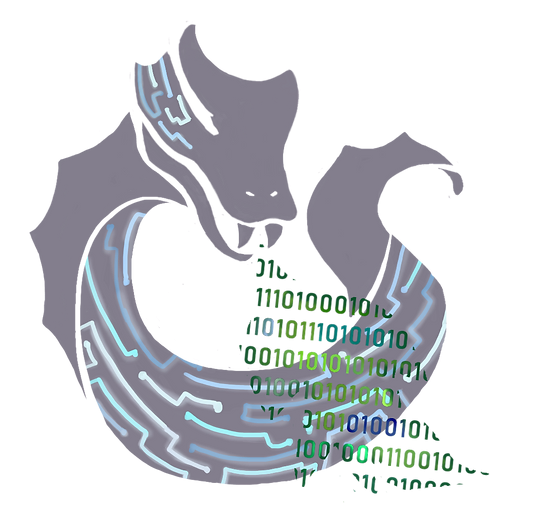
\includegraphics[width=0.25\textwidth,height=\textheight]{csclublogo.png}



\end{document}
